% ---------------------------------------------------------------------------
%  The combination rule, drawn as a picture of equation (2) of the paper.
%  Generated/hand-written for the companion; see ../code/gen_tikz.py.
% ---------------------------------------------------------------------------
\begin{figure}[H]
\centering
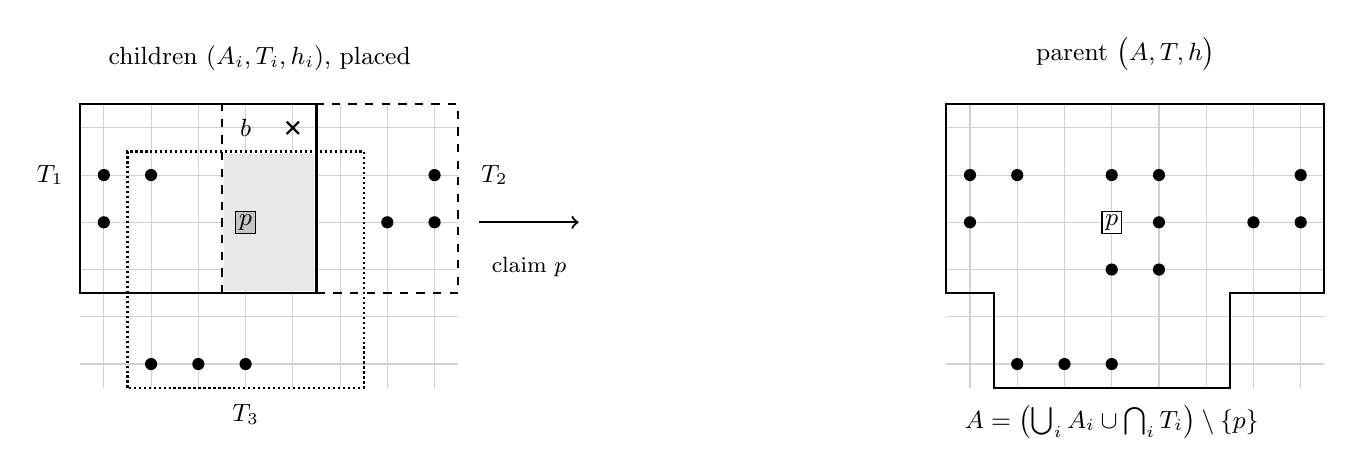
\begin{tikzpicture}[x=6mm,y=6mm,font=\small]
% ======================= left: three placed children ======================
\begin{scope}
 \draw[gray!35,step=1] (-4.5,-3.5) grid (3.5,2.5);
 % the three envelopes
 \draw[thick] (-4.5,-1.5) rectangle (0.5,2.5);
 \draw[thick,dashed] (-1.5,-1.5) rectangle (3.5,2.5);
 \draw[thick,densely dotted] (-3.5,-3.5) rectangle (1.5,1.5);
 % their common part
 \fill[gray!18] (-1.45,-1.45) rectangle (0.45,1.45);
 % required cells of the children
 \foreach \x/\y in {-4/0,-4/1,-3/1}{\fill (\x,\y) circle (2.2pt);}
 \foreach \x/\y in {2/0,3/0,3/1}{\fill (\x,\y) circle (2.2pt);}
 \foreach \x/\y in {-3/-3,-2/-3,-1/-3}{\fill (\x,\y) circle (2.2pt);}
 % the pivot, and one Breaker stone
 \node[draw,fill=gray!45,inner sep=1.2pt] at (-1,0) {$p$};
 \draw[thick] (-.13,1.87)--(.13,2.13) (-.13,2.13)--(.13,1.87);
 % labels
 \node[left] at (-4.65,1) {$T_1$};
 \node[right] at (3.78,1) {$T_2$};
 \node[below] at (-1,-3.65) {$T_3$};
 \node at (-1,2) {$b$};
 \node[above] at (-.7,3.0) {children $(A_i,T_i,h_i)$, placed};
\end{scope}
% ======================= right: the parent card ===========================
\begin{scope}[xshift=11cm]
 \draw[gray!35,step=1] (-4.5,-3.5) grid (3.5,2.5);
 % the envelope {p} u U T_i
 \draw[thick] (-4.5,2.5)--(-4.5,-1.5)--(-3.5,-1.5)--(-3.5,-3.5)--(1.5,-3.5)
              --(1.5,-1.5)--(3.5,-1.5)--(3.5,2.5)--cycle;
 % U A_i u (n T_i) minus the pivot
 \foreach \x/\y in {-4/0,-4/1,-3/1,2/0,3/0,3/1,-3/-3,-2/-3,-1/-3,
                    -1/-1,0/-1,-1/1,0/0,0/1}{\fill (\x,\y) circle (2.2pt);}
 \node[draw,fill=white,inner sep=1.2pt] at (-1,0) {$p$};
 \node[above] at (-.7,3.0) {parent $\bigl(A,T,h\bigr)$};
 \node[below] at (-1,-3.65) {$A=\bigl(\bigcup_iA_i\cup\bigcap_iT_i\bigr)\setminus\{p\}$};
\end{scope}
\draw[->,thick] (3.95,0)--(6.05,0);
\node[font=\footnotesize] at (5.0,-0.95) {claim $p$};
\end{tikzpicture}
\caption{The combination rule, Lemma~3 of the paper. Left: the children,
placed in one frame. The shaded block is $\bigcap_iT_i$; the pivot $p$
lies in it; Section~\ref{sec:pivot} says what a pivot is. Maker claims $p$, which makes every $A_i$ and the whole shaded block
Maker's. Because $p\in T$ and $T_i\subseteq T$, Breaker owns no cell of any
$T_i$; its next stone $b$ cannot be in every envelope --- here $b\notin T_3$ ---
so at least one child is still available. Right: the parent card. Its envelope
is $\{p\}\cup\bigcup_iT_i$ and its required set is the union of the child
requirements together with the common block, with the pivot spent; its height
is $1+\max_ih_i$. Nothing is assumed about Maker cells outside
$\bigcup_iA_i\cup\bigcap_iT_i$, or about Breaker cells outside the envelope.}
\label{fig:combination}
\end{figure}
